\documentclass[11pts]{report}

\usepackage{qtree}
\usepackage{listings}
\usepackage{amsmath,mathtools}
\usepackage[ruled,longend]{algorithm2e}
\usepackage{tikz}
\usepackage{listings}
\usepackage{graphicx}
\usepackage{xcolor}
\lstset{
    frame=tb, % draw a frame at the top and bottom of the code block
    tabsize=4, % tab space width
    showstringspaces=false, % don't mark spaces in strings
    commentstyle=\color{green}, % comment color
    keywordstyle=\color{blue}, % keyword color
    stringstyle=\color{red} % string color
}

\title{CS 677 Homework \\ Assignment 05}
\date{October 3, 2018}
\author{\textbf{Hai Nguyen}}

\setlength{\topmargin}{-1cm}
\setlength{\oddsidemargin}{0in}
\setlength{\textwidth}{6.5in}
\setlength{\textheight}{8.3in}

\DeclareMathOperator{\Div}{div}
\newcommand{\vect}[1]{\mathbf{#1}}




%%Currently default settings for indentation and symbols.
%%Try these by uncommenting this block!!!
%%Redefine the first level symbols
%\renewcommand{\theenumi}{\fnsymbol{enumi}-}
%\renewcommand{\labelenumi}{\theenumi}
%
%%Redefine the second level symbols
%\renewcommand{\theenumii}{\alph{enumii})}
%\renewcommand{\labelenumii}{\theenumii}
%
%%Redefine the third level symbols
%\renewcommand{\theenumiii}{\roman{enumiii}.}
%\renewcommand{\labelenumiii}{\theenumiii}
%
%%Options for redefining levels


%\arabic
%\alph 
%\Alph
%\roman
%\Roman
%\fnsymbol
%This ^^^ is all you need to change!!

\begin{document}

\maketitle

\begin{enumerate}

% Question 1
\item 
\begin{enumerate}
\item Illustrate the operation of BUILD-MAX-HEAP on the array A = [5, 3, 17, 10, 84, 19, 6, 22, 9].

The operation is shown in Figure \ref{Fig:1a}.

\begin{figure}[htbp]
\begin{center}
\includegraphics[scale=0.5]{1a.png}
\caption{Illustration of BUILD-MAX-HEAP.}
\label{Fig:1a}
\end{center}
\end{figure}


\item Illustrate the operation of COUNTING-SORT on the array A = [6, 0, 2, 0, 1, 3, 4, 6, 1, 3, 2]

The operation is shown in Figure \ref{Figure:1b}.
\end{enumerate}
\begin{figure}[htbp]
\begin{center}
\includegraphics[scale=0.4]{1b.png}
\caption{Illustration of COUNTING-SORT.}
\label{Figure:1b}
\end{center}
\end{figure}

\item Suppose that we were to write the \textbf{for} loop header in line 10 of the COUNTING-SORT as 
\par 10 \quad \textbf{for} j = 1 \textbf{to} A.\textit{length}
\par Show that the algorithm still works properly. Is the modified algorithm stable?
\par \textbf{for} \textit{j} = A.\textit{length} \textbf{downto} 1
\par \quad B[C[A[$j$]]] = A[$j$]
\par \quad C[A[$j$]] = C[A[$j$]] - 1
\par The main purpose of the loop is to place each element A[\textit{j}] into its correct sorted position in the output array B. If n elements are distinct, then for each A[\textit{j}] the value C[A[$j$]] is the correct final position of A[$j$] in the output array, since there are C[A[$j$]] elements less than or equal to A[$j$]. Because the elements might not be distinct, we decrement C[A[$j$]] each time we place a value A[$j$] into the B array. Decrementing C[A[$j$]] causes the next input element with a value equal to A[$j$], if one exists, to go to the position immediately before A[$j$] in the output array. 

\par Therefore, we see that the correct position of A[$j$] in the output array is independent on the direction of j in the loop in line 10, which guarantees the correctness of the modified algorithm. When we increase j, the next element with a value equal to a previous A-front (labelled A-back) will still be right before the location of A-front in the output array due to decremented index. However, in the input array, A-front is before A-back. The reversed order makes the algorithm to be unstable.
\item Implement in C/C++ an algorithm that checks if an array of n elements is a heap and determine its running time. The algorithm should print “YES, heap” or “Not a heap”, depending on the outcome. Show how your algorithm works on the
following arrays A = [16 14 10 8 7 9 3 2 4 1] and B = [10 3 9 7 2 11 5 1 6].

\par Source code:

\begin{lstlisting}
#include <stdio.h> 
  
void printArray(int arr[], int n) 
{ 
    for (int i = 0; i < n; i++) 
        printf("%d ", arr[i]); 
}

void checkHeap(int arr[], int n) 
{ 
    int parent = 0;
    int left_child = 0;
    int right_child = 0;

    bool isHeap = true;

    for (int i = 0; i < n/2; i++)
    {
        parent = arr[i];
        left_child = arr[2 * i];
        right_child = arr[2 * i + 1];

        if ((parent < left_child) || (parent < right_child))
        {
            isHeap = false;
            break;
        }
    } 

    printArray(arr, n);
    
    if (isHeap)
    {
        printf("YES, heap\n");
    }
    else
    {
        printf("Not a heap\n");
    }

}

  
int main() 
{ 
    int arr1[] = { 16, 14, 10, 8, 7, 9, 3, 2, 4, 1 }; 
    int arr2[] = {10, 3, 9, 7, 2, 11, 5, 1, 6};
    checkHeap(arr1, sizeof(arr1) / sizeof(arr1[0]));
    checkHeap(arr2, sizeof(arr2) / sizeof(arr2[0]));
    return 0; 
} 
\end{lstlisting}

\par Outputs:
\begin{lstlisting}
16 14 10 8 7 9 3 2 4 1 YES, heap
10 3 9 7 2 11 5 1 6 Not a heap
\end{lstlisting}

\item Why do we want the loop index \textit{i} in line 2 of BUILD-MAX-HEAP to decrease from $\lfloor$A.length/2$\rfloor$ to 1 rather than increase from 1 to $\lfloor$A.length/2$\rfloor$.

\par BUILD-MAX-HEAP (A)
\par A.\textit{heap-size} = A.\textit{length}
\par \textbf{for} \textit{i} = $\lfloor$A.\textit{length/s}$\rfloor$ \textbf{downto} 1
\par \quad \quad MAX-HEAPIFY(A, $i$)

\par Because it is required for MAX-HEAPIFY to work properly. When MAX-HEAPIFY is called, it assumes that the binary trees rooted at LEFT($i$ and RIGHT($i$) are max-heaps. When we go bottom up, we have the loop invariant that at the start of each iteration of the for loop, each node $i$ + 1, $i$ + 2, ..., $n$ is the root of a max-heap. This allows MAX-HEAPIFY to work correctly when it is called. However, when we go in the opposite direction, the loop invariant does not hold anymore making the assumption invalid.
\item Describe an algorithm that, given $n$ integers in range 0 to $k$, preprocesses its input and then answers any query about how many of the $n$ integers fall into a range [a..b] in O(1) time. Your algorithm should use $\Theta(n + k)$ preprocessing time.

\par For $n$ given integers in range 0 to $k$, we preprocess them similarly when using COUNTING-SORT to have the array C[0..$k$] so that C[$i$] holds the number of input elements equal to \textit{i} for each integer \textit{i} = 0, 1, ..., \textit{k}. In this pre-processing step, to get C, we need $\Theta$(n + k) time. After we have the array C, there are different cases to answer the query, each takes a constant time:

\begin{itemize}
\item b $\leq$ a: Invalid case
\item a $<$ b:
	\begin{itemize}
	\item a $<$ b $\leq$ 0: Return 0
	\item a $\leq$ 0 $<$ b $\leq$ k: Return C[b]
	\item a $\leq$ 0 $<$ k $\leq$ b: Return n
	\item 0 $<$ a $<$ b $\leq$ k: Return C[b] - C[a-1]
	\item 0 $<$ a $<$ k $\leq$ b: Return C[k] - C[a-1]
	\end{itemize}
\end{itemize}

\item 
\begin{enumerate}
\item Find the smallest and the largest number of keys that a heap height $h$ can have.

\par From the definition of heap, Figure \ref{Figure:6a} shows when the heap has minimum and maximum number of keys.
\par Minimum number of keys: When the heap is a complete binary tree till height (\textit{h}-1) and has only one node at level \textit{h}.
\begin{align*}
m = 2^0 + 2^1 + ... + 2^{h-1} + 1 = 2^h
\end{align*}

\par Maximum number of keys: When the heap is a complete binary tree of height \textit{h}.
\begin{align*}
M = 2^0 + 2^1 + ... + 2^{h} = 2^{h+1} - 1
\end{align*}

\begin{figure}[htbp]
\begin{center}
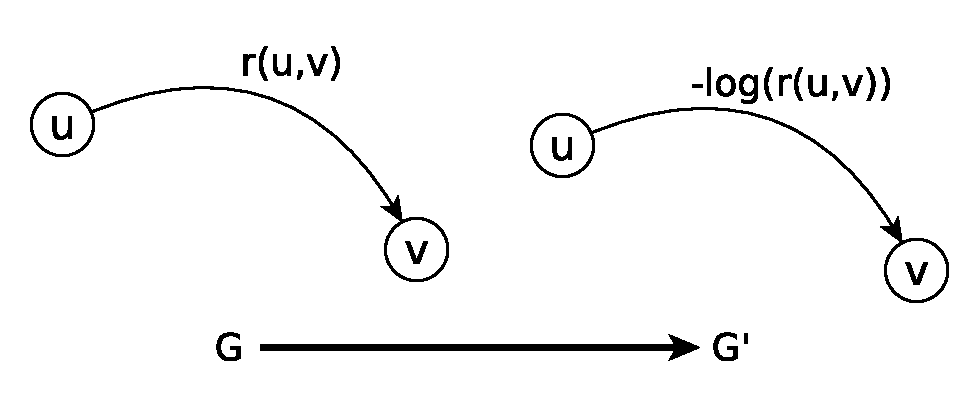
\includegraphics[scale=0.5]{6.png}
\caption{Cases with minimum and maximum number of keys.}
\label{Figure:6a}
\end{center}
\end{figure}

\item Prove that the height of a heap with \textit{n} nodes is $\lfloor$lgn$\rfloor$.
\par From (a) we have:
\begin{align*}
m &\leq n \leq M \\
2^h &\leq n \leq 2^{h+1} - 1 \\
2^h &\leq n < 2^{h+1} \\
h &\leq lgn \leq{h+1} \\
\to h &= \lfloor lgn \rfloor
\end{align*}

\end{enumerate}
\end{enumerate}

\end{document}
